\documentclass[11pt,letterpaper]{article}
\usepackage[T1]{fontenc}
\usepackage{lmodern,amsmath,amssymb,amsthm,mathtools,booktabs,graphicx}
\usepackage[margin=1in,top=.84in,bottom=.82in]{geometry}
\usepackage[final]{microtype}
\usepackage{xcolor,fancyhdr,enumitem}
\usepackage[hidelinks]{hyperref}
\definecolor{inkblue}{HTML}{17465A}
\hypersetup{colorlinks=true,linkcolor=inkblue,citecolor=inkblue,urlcolor=inkblue,pdftitle={Gaussian prime races: a transition modulo four and full-dimensional limit laws}}
\pagestyle{fancy}\fancyhf{}\fancyhead[L]{\small\textcolor{inkblue}{Gaussian prime races}}\fancyhead[R]{\small November 2026}\fancyfoot[C]{\thepage}
\setlength{\headheight}{14pt}
\setlist{topsep=3pt,itemsep=3pt}
\newtheorem{theorem}{Theorem}[section]
\newtheorem{lemma}[theorem]{Lemma}
\newtheorem{corollary}[theorem]{Corollary}
\newtheorem{proposition}[theorem]{Proposition}
\newcommand{\R}{\mathbb R}\newcommand{\C}{\mathbb C}\newcommand{\T}{\mathbb T}
\newcommand{\e}{\mathrm e}\newcommand{\dd}{\,\mathrm d}
\newcommand{\PP}{\mathcal P}\newcommand{\QQ}{\mathcal Q}
\DeclareMathOperator{\supp}{supp}
\newcommand{\abs}[1]{\left|#1\right|}
\setlength{\emergencystretch}{2em}
\begin{document}
\begin{center}
{\small\textsf{\textcolor{inkblue}{ANALYTIC NUMBER THEORY}}}\\[8pt]
{\huge\bfseries Gaussian prime races}\\[6pt]
{\large A transition modulo four and full-dimensional limit laws}\\[8pt]
{\small Research note \quad$\cdot$\quad 26 November 2026}
\end{center}
\begin{abstract}
Count primes in a moving Gaussian window on the logarithmic axis, weighting each prime by \((\log p)/\sqrt p\). We prove that the race between the classes \(3\) and \(1\) modulo \(4\) has a unique critical smoothing time in the certified interval \((0.04007656562,0.04007656609)\). Below it each class leads with positive logarithmic density. Above it the class \(3\) leads at every sufficiently large scale. At the threshold the class \(3\) leads with logarithmic density one. For arbitrary moduli we classify the transitions for every pair of classes by their limiting mean. Distinct inverse classes each win with density one half for every width. Every nonzero real projection has a limiting density and a uniform local occupation bound. For \(d=\varphi(q)\), adding the vectors at \(d\) distinct log-scales \(n^{\alpha_j}\), \(1<\alpha_j<2\), gives a single sequence with a limiting density in \(L^{1+\delta}(\mathbb R^d)\). The number-theoretic input is Dirichlet GRH. Multiplicities, coincidences, and rational relations among zero ordinates are allowed.
\end{abstract}

\section{The prime statistic and its laws}
Write \(G=(\mathbb Z/q\mathbb Z)^\times\), \(d=|G|\), with \(q\ge1\) and the one-element group for \(q=1\). For \(h>0\) and \(a\in G\), define
\begin{align}
 k_h(u)&=(4\pi h)^{-1/2}\exp(-u^2/(4h)),\nonumber\\
 \PP_a(t)&=\sum_{p\equiv a\ (q)}\frac{\log p}{\sqrt p}\,k_h(t-\log p)
                  -\frac{\exp(t/2+h/4)}{d},\label{eq:P}\\
 \QQ_a(t)&=\sum_{n\equiv a\ (q)}\frac{\Lambda(n)}{\sqrt n}\,k_h(t-\log n)
                  -\frac{\exp(t/2+h/4)}{d}.\label{eq:Q}
\end{align}
Here \(p\) runs through primes and \(\Lambda(p^k)=\log p\) for \(k\ge1\), with \(\Lambda=0\) elsewhere. At \(x=\e^t\) the window has fixed multiplicative width around \(x\). The subtracted term comes from the pole at \(s=1\); it cancels in pairwise races. All \(d\) classes are retained, so the total prime-count fluctuation is still present.

For the prime-only difference \(B_h=\PP_3-\PP_1\) modulo four, the threshold is pinned down by
\[
                 \boxed{\,0.04007656562<h_*<0.04007656609\,}.
\]
At \(h=0.040\) each class therefore leads with positive logarithmic density. At \(h=0.041\) class \(3\) leads at every sufficiently large scale. Theorem~\ref{th:transition} and Proposition~\ref{prop:enclosure} prove these assertions. The estimate in \eqref{eq:rate} controls the losing density up to the threshold.

For a vector process \(X(t)\), its logarithmic limiting law is the weak limit of the image of \(T^{-1}\dd t\) on \([0,T]\) under \(t\mapsto X(t)\). For a sequence, use its empirical measures. Write \(|B|\) for Lebesgue measure in the dimension of \(B\).

\begin{theorem}[Local occupation and projection densities]\label{th:local}
For \(X=\PP\) or \(\QQ\), there are an integer \(K\ge2\), \(C<\infty\), and \(T_0\), depending on \(q,h\), such that for every \(T\ge T_0\), unit \(v\in\R^d\), and Borel \(B\subset\R\),
\begin{equation}
 |\{t\in[T,T+1]:v\cdot X(t)\in B\}|\ \le\ C|B|^{1/K}.\label{eq:occupation}
\end{equation}
The logarithmic limiting law \(\mu_X\) exists and has compact support. Its projection in every unit direction satisfies the same bound, with a density uniformly bounded in \(L^p(\R)\) for each \(1\le p<K/(K-1)\). Its joint Fourier transform satisfies
\(\abs{\widehat\mu_X(\xi)}\le C(1+\|\xi\|)^{-1/K}\).
\end{theorem}

\begin{theorem}[A full-dimensional density from one sequence]\label{th:several}
Fix \(1<\alpha_1<\cdots<\alpha_m<2\). For \(X=\PP\) or \(\QQ\), the sequence
\begin{equation}
 S_n=\sum_{j=1}^m X(n^{\alpha_j})\qquad(n=1,2,\ldots)\label{eq:Sn}
\end{equation}
has limiting law \(\mu_X^{*m}\). At \(m=d\) this measure has a density in \(L^{1+\delta}(\R^d)\) for some \(\delta=\delta(q,h)>0\), and the same holds for \(m>d\). At \(m>K(d+\ell)\) it has a \(C^\ell\) density for every nonnegative integer \(\ell\) meeting this inequality. The scales can be chosen without knowledge of any zero.
\end{theorem}

For example, modulo \(4\) there are two reduced classes. Adding their two-component vectors at \(t=n^{4/3}\) and \(t=n^{5/3}\) gives a limiting law with a density in the plane. Theorems~\ref{th:transition} and \ref{th:generaltransition} describe the outcome at a single scale. As \(h\) increases, the ordinary-prime race undergoes a sharp change from recurrent reversals to an eventual permanent lead.

\paragraph{Mathematical inputs and precedent.}
The Lean development \cite{sernau} exports Mathlib's RH and a zero-free right half-plane for every Dirichlet character, with the principal pole excepted. Its readable edition derives a one-sided estimate on prime sums by putting lower and upper bounds on the same corrected covolume. A Mellin argument then excludes zeros. The original formalization and its verification are described in the Lean FRO--Mathlib statement \cite{lean} and the historical account \cite{wiki}. We use the zero-location endpoint to pass in the reverse direction, from zeros to a prime statistic. The results below are proved in ordinary mathematics.

The ProveIt synthesis \cite{proveit} combines 61 research packets. In its section on zeros and prime races, the theorem labelled \texttt{zer:thm:rank} obtains full rank of zero-multiplicity vectors even in short height intervals, using a Landau formula related to Banks \cite{banks}. Another theorem there places a ball in the convex hull of race values on multiplicative intervals. We use the insight that coincident zeros can still detect every direction. Lemma~\ref{le:rank} supplies the weaker global rank that suffices here with a separate proof. The later packets on filtered races and multiscale covariance study excursions and correlations at fixed lags. Our observation times in \eqref{eq:Sn} grow at distinct rates.

Rubinstein--Sarnak \cite{rs}, Akbary--Ng--Shahabi \cite{ans}, Devin \cite{devin} and Martin--Ng \cite{mn} study limiting distributions and ties in prime races. Devin's nonconcentration result for finite trigonometric sums and Lawton's small-value bound for scalar functions with bounded Fourier spectrum \cite{lawton} are particularly close. Analytic pushforward integrability is a general subject \cite{ghs}. The proposed contributions concern the threshold for the Gaussian race, local occupation of sets for its infinite spectrum, the broad-window exponent, and the full-dimensional law for \eqref{eq:Sn}. Section~\ref{sec:four} compares the transition with earlier work on smoothed races. Historical priority for the exact results remains open.
\section{A differentiated explicit formula}
For each character \(\chi\bmod q\) let \(\chi^*\) be its primitive inducer. Write \(m_\chi(\gamma)\) for the multiplicity at \(1/2+i\gamma\) of \(L(s,\chi^*)\), taking zero for absence. GRH places every nontrivial zero on this line. Let \(\Gamma\) be the union of the distinct positive ordinates and define
\[
 b_\gamma(a)=-\frac1d\sum_{\chi\bmod q}\overline{\chi(a)}\,m_\chi(\gamma)
 \qquad(\gamma\in\Gamma\cup(-\Gamma)\cup\{0\}).
\]
Conjugating the characters gives \(b_{-\gamma}=\overline{b_\gamma}\), and \(b_0\) is real. Put \(r_q(a)=|\{b\in G:b^2=a\}|\) and
\[
 F(t)=b_0+2\operatorname{Re}\sum_{\gamma\in\Gamma}b_\gamma\e^{-h\gamma^2}\e^{i\gamma t}.
\]

\begin{proposition}\label{pr:explicit}
For each fixed derivative order \(k\ge0\), as \(t\to\infty\),
\begin{equation}
 (\QQ-F)^{(k)}(t)=O_{q,h,k}(\e^{-t/4}),\qquad
 \left(\PP-F+\frac{r_q}{2d}\right)^{(k)}(t)=o_{q,h,k}(1).\label{eq:asymp}
\end{equation}
The exponential series, written with both signs before complexifying \(t\), converges normally on every bounded horizontal strip, together with all derivatives.
\end{proposition}
\begin{proof}
Gaussian inversion writes the prime-power sum twisted by \(\chi\) as
\[
 \frac1{2\pi i}\int_{\Re s=2}
 \frac{-L'(s,\chi)}{L(s,\chi)}
 \exp\{h(s-\tfrac12)^2+t(s-\tfrac12)\}\dd s.
\]
Move to \(\Re s=1/4\). The standard local partial-fraction formula and the unit-interval zero count \(O_q(\log(2+|u|))\) give a logarithmic bound for \(L'/L(1/4+iu,\chi)\) for large \(|u|\), since critical zeros have horizontal distance \(1/4\). Imprimitive Euler factors have zeros on \(\Re s=0\) and bounded logarithmic derivatives in the strip used here. Choose horizontal sides in \([N,N+1]\) and \([-N-1,-N]\) at distance \(\gg_q1/\log N\) from nearby ordinates. The logarithmic derivative on these sides is \(O_q(\log^2 N)\). These estimates follow from the Dirichlet \(L\)-function partial fractions in \cite{kouk}. The Gaussian makes the horizontal integrals tend to zero even after inserting \((s-1/2)^k\).
The new vertical line contributes \(O_{q,h,k}(\e^{-t/4})\). Each critical zero contributes its negative multiplicity times \(\exp(-h\gamma^2+i\gamma t)\), and the principal pole contributes \(\exp(h/4+t/2)\), before differentiation. Character orthogonality gives the first formula. The local zero count proves normal convergence.

The terms \(p^j\) with \(j\ge3\) have total absolute coefficient at most
\(\sum_p(\log p)p^{-3/2}/(1-p^{-1/2})<\infty\), so their translated Gaussian and each derivative tend to zero. For squares in class \(a\), each class \(b\) with \(b^2=a\) contributes
\[
 \sum_{p\equiv b\ (q)}\frac{\log p}{p}\,k_h^{(k)}(t-2\log p).
\]
The prime number theorem in progressions and partial summation show that the measure
\(\sum_{p\equiv b\ (q)}(\log p)p^{-1}\delta_{2\log p}\), shifted left by \(t\), gives mass tending to \((B-A)/(2d)\) on each fixed interval \([A,B]\). Indeed the endpoints for \(p\) are \(\exp((t+A)/2)\) and \(\exp((t+B)/2)\); substitute \(\vartheta(y;q,b)=y/d+o_q(y)\) in partial summation on that interval. The mass of every translated unit interval is bounded by the Chebyshev bound \(\vartheta(y)\ll y\). Gaussian decay therefore permits passage from interval tests to \(k_h^{(k)}(-u)\) by truncation and uniform approximation. Its integral is one for \(k=0\) and zero otherwise. Summing over square roots proves the second formula.
\end{proof}

\begin{lemma}[No constant direction]\label{le:rank}
For every real \(v\ne0\), some \(\gamma>0\) satisfies \(v\cdot b_\gamma\ne0\). More generally, if complex \(c_\chi\) satisfy \(\sum_\chi c_\chi m_\chi(\gamma)=0\) for every nonzero signed ordinate, all \(c_\chi\) vanish.
\end{lemma}
\begin{proof}
Use the entire order-one completion
\[
 \Xi_\chi(s)=[s(s-1)]^{\delta_\chi}
 (f_\chi/\pi)^{(s+a_\chi)/2}\Gamma((s+a_\chi)/2)L(s,\chi^*),
\]
where \(f_\chi\) is the conductor, \(a_\chi\in\{0,1\}\) the parity, and \(\delta_\chi=1\) for the conductor-one principal character only. Its zeros are exactly the nontrivial zeros, with multiplicity. The genus-one Hadamard product gives
\[
 \sum_\chi c_\chi\,\frac{\Xi_\chi'}{\Xi_\chi}(s)= A+\frac{M}{s-1/2},
 \qquad M=\sum_\chi c_\chi m_\chi(0).
\]
Indeed the grouped terms \(1/(s-\rho)+1/\rho\) converge normally off the zeros; all noncentral groups cancel. Put \(D(s)=\sum c_\chi L'(s,\chi^*)/L(s,\chi^*)\). Subtract the identity at \(s\) from that at \(s+2\). The conductor constants disappear and the logarithmic gamma derivatives differ by \(1/(s+a_\chi)\), including the factor \(1/2\) from the chain rule. The factors \(s(s-1)\) contribute rational terms. Hence \(D(s+2)-D(s)\) is rational. The Euler series gives \(D(\sigma)=O(2^{-\sigma})\) as \(\sigma\to+\infty\) for fixed coefficients. A rational function with this decay on the positive real axis vanishes identically. Iterating the period \(2\) gives \(D=0\) for real \(s>1\). Uniqueness of Dirichlet coefficients gives \(\sum c_\chi\chi(p)=0\) at every prime \(p\nmid q\). Each reduced class contains a prime, and the character table is invertible. For real \(v\), annihilation at positive ordinates implies annihilation at negative ordinates by conjugation. Apply the stronger assertion to \(c_\chi=\sum_a v_a\overline{\chi(a)}\) and invert the character table again.
\end{proof}

\section{Every projection spends little time in small sets}
Let \(H\) be the closure of the orbit \(\theta_t=(\e^{i\gamma t})_{\gamma\in\Gamma}\) in the product of unit circles. This compact abelian group retains all arithmetic relations among the ordinates. Let \(\nu\) denote its normalized Haar measure. For \(z\in H\), put
\[
 F_z(t)=b_0+2\operatorname{Re}\sum_{\gamma>0}
                 b_\gamma\e^{-h\gamma^2}z_\gamma\e^{i\gamma t}.
\]
Every derivative is continuous in \((z,t)\), and all \(F_z\) are real analytic. Translation satisfies \(F_z(t+u)=F_{z\theta_u}(t)\). A finite product of coordinate characters restricts on the orbit to \(\e^{i\omega t}\); it is nontrivial on \(H\) precisely when \(\omega\ne0\). Continuous-time averaging kills these nontrivial characters. Their finite linear combinations are uniformly dense in \(C(H)\) by Stone--Weierstrass. Hence the law of \(\QQ\) is the image of \(\nu\) under \(z\mapsto F_z(0)\) and the law of \(\PP\) is its translate by \(-r_q/(2d)\), by \eqref{eq:asymp}. In particular their means are \(b_0\) and \(b_0-r_q/(2d)\).

\begin{lemma}[Uniform derivative order]\label{le:type}
There are \(K\ge2\) and \(c>0\) such that for every \(z\in H\), real unit \(v\), and real \(t\),
\[
 \max_{1\le j\le K}|v\cdot F_z^{(j)}(t)|\ge c .
\]
\end{lemma}
\begin{proof}
If \(v\cdot F_z\) were constant on any interval, analyticity would make it constant on the line. Multiplication by \(\e^{-i\gamma t}\) and averaging would give \(v\cdot b_\gamma=0\) at every positive frequency, contradicting Lemma~\ref{le:rank}. Thus at \(t=0\) at least one positive-order derivative is nonzero for every \((v,z)\). Compactness of the unit sphere times \(H\), and continuity, give a finite cover, a common maximum order and a strictly positive lower bound. Translation supplies every \(t\).
\end{proof}

\begin{lemma}[Occupation on a real interval]\label{le:occ}
Consider \(C^{K+1}\) real functions \(g\) on intervals of length one. Suppose their derivatives of orders \(1,\ldots,K+1\) are uniformly bounded and \(\max_{1\le j\le K}|g^{(j)}|\ge c>0\) pointwise. Uniformly in \(g\), Borel \(B\subset\R\), and real \(u\), one has
\[
 |\{t:g(t)\in B\}|\ll |B|^{1/K},\qquad
 \left|\int \exp(iu g(t))\dd t\right|\ll(1+|u|)^{-1/K}.
\]
\end{lemma}
\begin{proof}
A sufficiently fine common mesh divides the interval into boundedly many pieces. On each piece some fixed \(|g^{(j)}|\ge c/2\) throughout, by the derivative bound at order \(j+1\). For \(j=1\) change variables directly. For \(j\ge2\), the set \(|g'|\le s\) has length \(O(s^{1/(j-1)})\). To see the elementary sublevel estimate used here, if \(|f^{(k)}|\ge c/2\) and \(|f|\le s\) on a set of length \(L>0\), choose \(k+1\) points of this set separated by \(\gg_k L\) using its measure quantiles. Their order-\(k\) divided difference has absolute value \(O_k(s/L^k)\) and equals \(f^{(k)}(\tau)/k!\). This proves the bound. On the complement of \(|g'|\le s\), the inverse change of variables gives at most \(j|B|/s\): Rolle's theorem bounds the number of monotone branches by \(j\). For \(0<|B|\le1\) take \(s=|B|^{(j-1)/j}\); null sets follow on letting \(s\downarrow0\), and large sets are immediate. Each interval contributes \(O(|B|^{1/j})\).
For the oscillatory integral use the order-\(j\) van der Corput lemma when \(j\ge2\). When \(j=1\), a single integration by parts uses the lower bound on \(|g'|\) and the upper bound on \(|g''|\). Summing over the mesh proves the assertions.
\end{proof}

\begin{proof}[Proof of Theorem~\ref{th:local}]
Apply the lemmas to \(g(t)=v\cdot F_z(t)\), allowing any additive constant. Proposition~\ref{pr:explicit} transfers the same hypotheses to each sufficiently late unit interval of the actual prime statistics: the error and its first \(K+1\) derivatives tend to zero for fixed \(q,h\), uniformly over all unit directions. This proves the local Borel bound. For the limiting measures average the estimates for \(F_z\) on \([0,1]\) over \(z\) and use Haar invariance. The Borel estimate gives absolute continuity; if \(w\) denotes the projected density, \(u|\{w>u\}|\le C|\{w>u\}|^{1/K}\). The resulting weak \(L^{K/(K-1)}\) estimate, compact support, and integration of level sets give the claimed strong \(L^p\) norms. Applying the oscillatory estimate in direction \(\xi/\|\xi\|\) gives the Fourier bound.
\end{proof}

In particular any finite list of strict linear inequalities in the smoothed races has a logarithmic density, since its boundary is contained in finitely many hyperplanes of measure zero. A specific density can be zero or one. Section~\ref{sec:four} gives an example where this distinction matters.

\section{A critical smoothing time for primes modulo four}\label{sec:four}

For the prime-only race put $B_h(t)=\PP_3(t)-\PP_1(t)$ at modulus $4$.
Let $\beta(s)=L(s,\chi_4)$ denote the Dirichlet beta function,
and let $\gamma_1$ be its least positive nontrivial zero ordinate.
The Gaussian width determines whether the class $1$ can lead at
arbitrarily large scales.

\begin{theorem}\label{th:transition}
There is a unique $h_*>0$ with the following transition. For every
$0<h<h_*$, each strict sign of $B_h$ occurs with positive limiting
density in $t=\log x$. For every $h>h_*$, $B_h(t)$ is bounded below
by a positive constant for all sufficiently large $t$. At $h=h_*$
the limiting density of $B_{h_*}(t)>0$ is one and
$\liminf_{t\to\infty}B_{h_*}(t)=0$. The transition satisfies
\[
                 \frac{\log 2}{\gamma_1^2}< h_* < \frac1{22}.
\]
\end{theorem}

Equivalently let \(R_h(X)\) denote the excess of class \(3\) over class \(1\) with unnormalized weights \((\log p)\exp[-(\log(p/X))^2/(4h)]\). The square completion gives
\[
 \frac{R_h(X)}{\sqrt{X}}=\sqrt{4\pi h}\,\e^{h/4} B_h(\log X+h).
\]
Hence, for \(h>h_*\), \(R_h(X)\ge c_h\sqrt X\) eventually for some \(c_h>0\). Below the threshold, each class has a lead of at least \(c_h\sqrt X\) on a set of positive logarithmic density, after choosing \(c_h>0\) sufficiently small.

Knapowski and Tur\'an proved eventual divergence of this weighted excess at the particular width \(h=1/4\) under GRH for \(\beta\) \cite{kt,bp,suzuki}. Neroli proves critical exponents and smoothing orders for exponential and iterated Mellin kernels \cite[Theorems 2.2 and 3.3]{neroli}. The positivity argument below shares the idea of averaging translates with that work. For logarithmic Gaussians the multiplier is exactly \(\exp(-h\gamma^2)\), which permits a certified enclosure for the transition and a bound on the density of reversals.

\begin{proof}
The alternating series gives $\beta(1/2)>0$. The squares of both
units modulo four are $1$, so removing the prime squares adds $1/2$
to the difference between classes $3$ and $1$. The prime-only
formula~\eqref{eq:asymp} gives
\[
 B_h(t)=f_h(\theta_t)+o(1),\qquad
 f_h(z)=\tfrac12+2\operatorname{Re}\sum_{\gamma>0}
                    m_\gamma e^{-h\gamma^2} z_\gamma .
\]
Here $m_\gamma$ is the multiplicity for $\beta$, and the compact
group $H$ is the closure of $\theta_t=(e^{i\gamma t})_{\gamma>0}$.
The sign of the sum follows from subtracting class $1$ from class
$3$, which takes the negative of the $\chi_4$ component of the
prime-weighted sum. Every orbit $z\theta_t$ is dense in $H$.
Every open neighborhood in $H$ has positive Haar measure and is
visited at arbitrarily large positive times. Consequently
$m(h):=\min_H f_h=\liminf_{t\to\infty} B_h(t)$.

The function $m(h)$ is continuous for $h>0$ by local uniform convergence.
For $u>0$ the heat semigroup gives the identity
\[
 f_{h+u}(z)=\int_{\mathbb R} k_u(v)f_h(z\theta_v)\,dv .
\]
The function $f_h$ is nonconstant, as its Fourier coefficient at
$\gamma_1$ is nonzero. Each orbit visits an open set where
$f_h>m(h)$, and $k_u$ is strictly positive. Thus
$f_{h+u}(z)>m(h)$ for each $z$, and compactness gives
$m(h+u)>m(h)$. As $h\to\infty$, $f_h\to1/2$ uniformly.

Suppose $f_h\ge0$. Its Haar integral is $1/2$, so
\[
 m_{\gamma_1}e^{-h\gamma_1^2}
 =\left|\int_H f_h(z)\overline{z_{\gamma_1}}\,dz\right|<\tfrac12.
\]
For strictness, equality in the integral triangle inequality would
force $z_{\gamma_1}$ to be constant almost everywhere on the set
where $f_h>0$, hence everywhere there by continuity and full support.
That set contains an orbit segment, on which the coordinate rotates
at nonzero speed. Since $m_{\gamma_1}\ge1$, this proves
$m((\log2)/\gamma_1^2)<0$.

It follows that $m(h_*)=0$ has exactly one solution. Below it, both
strict sign sets are open and nonempty on $H$, since the mean is
positive. The projection has an absolutely continuous limiting law,
so $f_h=0$ has measure zero and contains the boundaries of both sign sets. Equidistribution
and the $o(1)$ approximation give the stated densities, including
density one at $h_*$. Above $h_*$ the positive minimum gives a uniform
margin at all sufficiently large times. The explicit upper endpoint
is proved next.
\end{proof}

\paragraph{An upper bound from two values of the completed logarithmic derivative.}
Write $D(s)=\Xi'(s)/\Xi(s)$ for
$\Xi(s)=(4/\pi)^{(s+1)/2}\Gamma((s+1)/2)\beta(s)$.
This is an entire function of order one, even about $s=1/2$.
The paired Hadamard product for
$\Xi(1/2+u)/\Xi(1/2)$ has factors
$(1+u^2/\gamma^2)^{m_\gamma}$ for $\gamma>0$.
Any linear exponential prefactor is constant by evenness.
Logarithmic differentiation at $u=1,2$ yields the positive moment
\[
 S:=\sum_{\gamma}\frac{m_\gamma}{(1+\gamma^2)(4+\gamma^2)}
       =\frac{D(3/2)-D(5/2)/2}{3}<0.00168 ,
\]
where both signs of each ordinate are included. For $y\ge0$,
\[
 (1+y)(4+y)e^{-y/22}\le(y+5/2)^2 e^{-y/22}
 \le44^2 e^{-83/44}<294 .
\]
Hence $\sum_\gamma m_\gamma e^{-\gamma^2/22}<294(0.00168)<1/2$.
This gives $m(1/22)>0$ uniformly over all phases, including any
relations among the ordinates.

For reproducibility, write $D(s)=A(s)+\beta'(s)/\beta(s)$. At
$s=3/2,5/2$ respectively the two values of $2A(s)-\log(4/\pi)$
are $4-\gamma_{\rm E}-\pi/2-3\log2$ and
$4/3-\gamma_{\rm E}+\pi/2-3\log2$, by digamma recurrence and reflection.
The partial alternating sums through $n=2047$ bound $\beta(3/2)$
from below and $\beta'(3/2)$ from above. Those through $2049$ bound
$\beta(5/2)$ from above and $\beta'(5/2)$ from below. Indeed
$(\log n)n^{-s}$ decreases for $n\ge3$ at either value of $s$,
and the derivatives of the constant terms vanish.
These rationally enclosable sums give $D(3/2)<0.15427$ and
$D(5/2)>0.29847$. The included \texttt{bound.py} checks the
inequalities with integer square roots and the series
$\log((1+u)/(1-u))=2\sum_{j\ge0}u^{2j+1}/(2j+1)$ after reduction
to $0\le u\le1/3$.

\paragraph{Direct arithmetic check.}
At $h=0.04$ the table compares the prime-power difference
$Q=\QQ_3-\QQ_1$, the prime-only difference $B=B_h$, and
the truncated zero sum $Z=2\sum_{0<\gamma\le32}
e^{-h\gamma^2}\cos(\gamma t)$ over the ten roots detected by
\texttt{verify.py}. The two classes have identical subtracted
main terms. The program sums odd prime powers up to $24\,154\,953$.
The integral majorant for the omitted arithmetic tail is less than
$1.2\times10^{-21}$ throughout the table. The ordinates were found
by a numerical sign scan, which supplies an illustration of the
formula. The upper bound for $h_*$ uses the separate rational certificate.

\begin{center}
\begin{tabular}{r@{\qquad}r@{\qquad}r@{\qquad}r@{\qquad}r}
\toprule
$t$ & $Q$ & $Z$ & $B$ & $B-Z-1/2$\\
\midrule
 6 & $ 0.002964$ & $ 0.002829$ & $0.341832$ & $-0.160996$\\
 8 & $-0.209244$ & $-0.209251$ & $0.339891$ & $ 0.049142$\\
10 & $-0.418259$ & $-0.418259$ & $0.060718$ & $-0.021023$\\
12 & $-0.495944$ & $-0.495944$ & $0.002424$ & $-0.001632$\\
14 & $-0.389047$ & $-0.389047$ & $0.119904$ & $ 0.008951$\\
\bottomrule
\end{tabular}
\end{center}

The first computed ordinate is about $6.02095$, placing the
symbolic lower bound near $0.01912$. Although class $3$ leads at all
five sample times, Proposition~\ref{prop:enclosure} proves that both
classes lead with positive logarithmic density at this width.

\subsection{A certified interval for the transition}
\label{sec:enclosure}

\begin{proposition}\label{prop:enclosure}
The critical Gaussian smoothing time modulo four satisfies
\[
                   0.04007656562<h_*<0.04007656609 .
\]
The interval has width $4.7\times10^{-10}$. In particular both classes lead with positive logarithmic density at
$h=0.04$.
\end{proposition}

\begin{proof}
The external numerical input consists of the first ten consecutive
positive ordinates of $\beta$, counted with multiplicity, and the fact
that the eleventh exceeds $32$. The LMFDB record for the primitive
character $4.3$ supplies the ordinates. Its reliability page specifies
interval-arithmetic accuracy to one unit in the last displayed place
and completeness through the range shown. The first and tenth
ordinates are approximately $6.0209489047$ and $29.6563840146$; the
eleventh is approximately $32.5921865271$. The certificate truncates
the ten entries to $22$ places after the decimal point and allows
error $10^{-21}$ at each center.%
\footnote{The LMFDB, \emph{Dirichlet $L$-function $1$-$2$e$2$-$4.3$-r$1$-$0$-$0$},
\url{https://www.lmfdb.org/L/1/2e2/4.3/r1/0/0}.
The linked Reliability and Source pages give the error and completeness
statements and attribute the computation to David Platt.}

For a short independent tail estimate, let $D$ denote the completed
logarithmic derivative from the preceding subsection. Its paired
Hadamard formula gives
\[
 \sum_{\gamma>0}\frac{m_\gamma}{9/4+\gamma^2}
   =\frac{D(2)}{3}<1.
\]
Indeed
$D(2)=\tfrac12\log(4/\pi)+\tfrac12\psi(3/2)+\beta'(2)/\beta(2)$,
where $\psi$ is the digamma function. The first two terms together
are less than one, since $\psi(3/2)<\psi(2)=1-\gamma_{\rm E}<1$.
The Euler series bounds the last term in absolute value by
$\sum_{n\ge2}(\log n)n^{-2}<2$, by comparison with its integral.
For either endpoint $h$ in the proposition, $(9/4+u^2)e^{-hu^2}$
decreases for $u\ge32$. Thus the absolute contribution of all
omitted harmonics is at most $2(9/4+32^2)e^{-h32^2}<4\cdot10^{-15}$.

Write $h_-=0.04007656562$, $h_+=0.04007656609$ and
$t_0=59260005815.44527175543962534$, all taken as exact rationals.
At $h_-$ the time $t_0$ supplies one admissible point of the compact
phase group. At $h_+$ the triangle inequality bounds every phase at
once. The complete enclosures, including the tail, are
\begin{align*}
 -2445384\cdot10^{-15}
 &\le \tfrac12+2\sum_{\gamma>0}m_\gamma
      e^{-h_-\gamma^2}\cos(\gamma t_0)
    \le-74977\cdot10^{-15},\\
 47190\cdot10^{-15}
 &\le \tfrac12-2\sum_{\gamma>0}m_\gamma e^{-h_+\gamma^2}
    \le47197\cdot10^{-15}.
\end{align*}
The first upper bound is negative and the second lower bound is
positive. Strict monotonicity of the minimum proves the claim.

The file \texttt{certify\_threshold.py} reproduces these inequalities
using integer and rational arithmetic. It encloses $\pi$ by
Machin's formula, reduces each cosine argument, and bounds the
Taylor remainders for the exponential and cosine. Moving any one
input ordinate within its radius $\varepsilon$ changes a doubled
summand by at most $2(64h+|t_0|)\varepsilon$; for the amplitude
bound one can set $t_0=0$ in this estimate. This accounts for
the amplification of ordinate errors at the large witness time.
\end{proof}

\begin{figure}[htb]
\centering
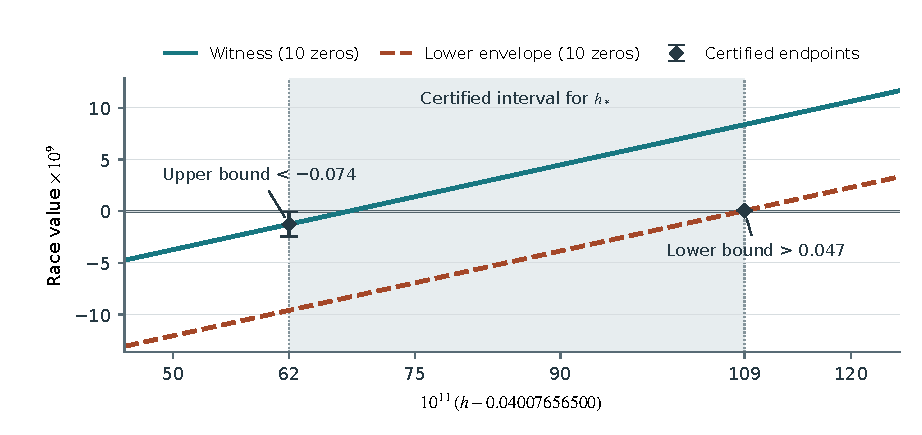
\includegraphics[width=.88\linewidth]{threshold_bounds.pdf}
\caption{Two bounds on the limiting minimum near its zero. The upper curve evaluates one time shared by all ten retained harmonics. The lower curve gives each harmonic its most negative possible value. The plotted curves use the ten-term sums. Diamonds mark the midpoints of the certified endpoint enclosures. The vertical bars include ordinate uncertainty and the full spectral tail. The bar at the right endpoint is smaller than its marker. Opposite strict signs certify the shaded interval.}
\end{figure}

\subsection{How fast the losing density vanishes}
Let \(p_-(h)\) be the logarithmic density of \(B_h(t)<0\). On \(I=[0.040,0.041]\), which contains the transition, there is a constant \(C\) such that
\begin{equation}
 |p_-(h)-p_-(h')|\le C|h-h'|^{1/2}\qquad(h,h'\in I).\label{eq:rate}
\end{equation}
Thus the losing density tends to zero at least as fast as \(C\sqrt{h_*-h}\) from below. This estimate addresses the frequency of reversals near the threshold.

To prove it, use the phase variable \(\theta=\gamma_1 t\) on any translated orbit and divide the centered signal by \(2\e^{-h\gamma_1^2}\). The first oscillation is a cosine with amplitude one. The total contribution of the remaining terms to each of its first two derivatives in \(\theta\) has magnitude at most
\[
 \frac{\sum_{\gamma>\gamma_1} m_\gamma\gamma^2\e^{-0.040\gamma^2}}
      {\gamma_1^2\e^{-0.041\gamma_1^2}} < \frac{2}{7}.
\]
Here the first ten certified ordinates and the tail estimate in Proposition~\ref{prop:enclosure} give numerator \(<2\) and denominator \(>7\). For the numerator's tail use
\(32^2(9/4+32^2)\exp(-0.040\cdot32^2)\) since
\(y(9/4+y)\exp(-0.040y)\) decreases for \(y\ge32^2\).
The extra lines in \texttt{certify\_threshold.py} verify both inequalities. The largest of the first two cosine derivatives has modulus at least \(1/\sqrt2\), and the third derivative is uniformly bounded for \(h\in I\). Lemma~\ref{le:occ} with \(K=2\) now gives \(\nu\{z:|f_h(z)|\le s\}\ll\sqrt{s}\) uniformly on \(I\); the amplitude and time normalizations stay in compact positive intervals. Termwise differentiation in \(h\) gives \(\|f_{h'}-f_h\|_\infty\ll|h'-h|\) on \(I\). A sign disagreement forces \(|f_h|\le\|f_{h'}-f_h\|_\infty\), proving \eqref{eq:rate}.

\section{The transition for every pair of residue classes}
\label{sec:generalthreshold}

Fix distinct $a,b\in G$ and write $B_h(t)=\mathcal P_a(t)-\mathcal P_b(t)$.
Its limiting mean
\[
 M=b_0(a)-b_0(b)-\frac{r_q(a)-r_q(b)}{2d}
\]
is independent of $h$. This includes possible central zeros.
\begin{theorem}\label{th:generaltransition}
If $M=0$, both signs of $B_h$ occur with positive logarithmic density
for every $h>0$. If $M\ne0$, there is a unique $h_*(a,b)>0$ below
which both signs have positive logarithmic density. Above it,
$\operatorname{sgn}(M) B_h$ is bounded below by a positive constant
at all sufficiently late times. At the threshold this oriented race
is positive with logarithmic density one and has lower limit zero.
\end{theorem}

\begin{proof}
Write $f_h$ for the prime-only difference on the phase group $H$,
so $B_h(t)=f_h(\theta_t)+o(1)$ as $t\to\infty$ for fixed $h$.
The semigroup argument of Theorem~\ref{th:transition} shows that
$\min_H f_h$ is strictly increasing and $\max_H f_h$ strictly decreasing:
Lemma~\ref{le:rank} ensures nonconstancy at every $h$.
Both extrema are continuous and converge to $M$ as $h\to\infty$.

To determine the other endpoint, take a prime $p\nmid q$ and put
$t_p=\log p$. We claim
\[
 f_h(\theta_{t_p})=
 \frac{\log p}{\sqrt{4\pi h p}}
  \bigl(\mathbf 1_{p\equiv a\,(q)}-\mathbf 1_{p\equiv b\,(q)}\bigr)
       +O_{p,q}(1) \qquad (h\downarrow0).
\]
This statement concerns the limiting phase function at the fixed time
$t_p$. To prove it, form the tempered distribution
$U_\chi(t)=-\sum_\gamma m_\chi(\gamma)e^{i\gamma t}$
over all signed ordinates, including zero. Temperedness follows from
the zero count. On the open half-line $t>0$, the explicit formula
for the primitive inducer gives the distribution identity
\[
 U_\chi=
 \sum_{n\ge2}\frac{\Lambda(n)\chi^*(n)}{\sqrt n}\,\delta_{\log n}
 -\delta_\chi e^{t/2}
 +\sum_{\omega\ {\rm trivial}}e^{(\omega-1/2)t}.
\]
The last sum runs over the actual trivial zeros of $L(s,\chi^*)$,
with multiplicity, and converges locally to an analytic function.
Indeed test on $\phi\in C_c^\infty(0,\infty)$ and insert
$\int\phi(t)e^{(s-1/2)t}\,dt$ in the logarithmic-derivative contour
of Proposition~\ref{pr:explicit}. Fourier inversion on $\Re s=2$
gives the prime-power atoms. Shift first to $\Re s=-N-1/2$ for an
integer $N$, taking admissible horizontal heights as in that proposition.
The poles and zeros give the terms displayed. On the new line the
functional equation and Stirling's estimate away from trivial zeros
bound $L'/L$ by $O_q(\log(2+N+|\Im s|))$. Integration by parts in the
test transform yields vertical decay of arbitrary fixed order with a
polynomial cost in $N$, times $e^{-N\inf\operatorname{supp}\phi}$.
The vertical remainder therefore vanishes as $N\to\infty$.

Take the character combination for $a-b$ and subtract the constant
prime-square shift. Convolution with $k_h$ gives exactly
$f_h(\theta_t)$ by its absolutely convergent Fourier series. Near
$t_p$ the distribution is a smooth function plus one point mass;
character orthogonality gives the coefficient in the claimed formula,
since $p\nmid q$. Localize by a smooth cutoff equal to one near $t_p$.
The smooth term contributes $O(1)$. The complementary tempered
distribution contributes $o(1)$ because every Schwartz seminorm of the
Gaussian translated to $t_p$ and multiplied by the complementary
cutoff tends to zero exponentially in $1/h$. This proves the claim.

Each of $a$ and $b$ contains a prime. Evaluating at one from each
class proves that the maximum tends to $+\infty$ and the minimum
to $-\infty$ as $h\downarrow0$. If $M\ne0$, orient the race by its
sign and apply strict monotonicity of the minimum. Every nonempty open
sign set has positive Haar mass, while a level set has zero mass by
Theorem~\ref{th:local}. This gives all density and endpoint assertions,
including the zero-mean case by nonconstancy.
\end{proof}

\begin{corollary}[Inversion symmetry]\label{cor:inversion}
If $a\ne a^{-1}$, each class in the prime race $a$ versus $a^{-1}$
leads with logarithmic density exactly $1/2$ for every $h>0$.
In particular this holds for $2$ versus $3$ modulo $5$.
\end{corollary}
\begin{proof}
The character formula gives
$b_\gamma(a^{-1})=\overline{b_\gamma(a)}$ for each signed ordinate,
and $b_0$ is real. Inversion bijects the square roots of $a$ with
those of $a^{-1}$. Thus $z\mapsto\overline z$ exchanges the two
prime-only coordinates on $H$, including their constant terms.
This group involution preserves Haar measure and reverses the
difference. The tie set has measure zero by Theorem~\ref{th:local}.
\end{proof}

\section{A deterministic sum with a density in all coordinates}
\begin{proof}[Proof of Theorem~\ref{th:several}]
First, the sequence
\((\theta_{n^{\alpha_1}},\ldots,\theta_{n^{\alpha_m}})\) is equidistributed in \(H^m\).
A nontrivial product character has phase \(f(n)=\sum_j\omega_j n^{\alpha_j}\) with at least one nonzero \(\omega_j\). Let \(\alpha\) be the largest active exponent. On \([N,2N]\), for large \(N\), \(|f''|\asymp N^{\alpha-2}\), the implied constants being allowed to depend on the character. The second-derivative estimate for exponential sums \cite{gk} gives a bound \(O(N^{\alpha/2}+N^{1-\alpha/2})=o(N)\), valid also on subintervals of this block. Dyadic decomposition and the character criterion give the assertion. In particular, the limit of \eqref{eq:Sn} is a convolution even when the frequencies within a single copy of \(H\) have rational relations.

Write \(\Psi_z(t)=F_z(t)\) in the prime-power case and \(\Psi_z(t)=F_z(t)-r_q/(2d)\) for primes. For \(m=d\), fix \(z=(z_1,\ldots,z_d)\in H^d\) and form the real analytic map
\[
 \Phi_z(u)=\sum_{j=1}^d\Psi_{z_j}(u_j),\quad
 D_z(u)=\det\big(F'_{z_1}(u_1),\ldots,F'_{z_d}(u_d)\big),\quad u\in[0,1]^d.
\]
The velocities of each curve span \(\R^d\) on every nonempty open interval. Otherwise a nonzero projection is constant there, contrary to Lemmas~\ref{le:rank} and \ref{le:type}. Select the columns successively, each outside the span of its predecessors. Thus \(D_z\) is not identically zero for any \(z\).

We give the uniform argument needed for \(L^{1+\delta}\). There are constants \(a,C>0\), independent of \(z\), such that
\begin{equation}
 |\{u\in[0,1]^d: |D_z(u)|\le s\}|\le Cs^a\qquad(0<s\le1).
 \label{eq:det}
\end{equation}
At every \((z,u)\) some finite derivative of \(D_z\), possibly of order zero, is nonzero by analyticity on \(\R^d\). A nonzero symmetric derivative tensor has a nonzero repeated directional derivative, by polarization. Joint continuity gives a product neighborhood in \(H^d\) and a Euclidean ball on which its magnitude stays bounded below by a positive constant for that one fixed direction and order. Compactness gives finitely many such neighborhoods. On each applicable ball slice its intersection with the unit cube by lines in its chosen direction; the slices are intervals. The divided-difference estimate in Lemma~\ref{le:occ} bounds the sublevel length by \(O(s^{1/j})\) for derivative order \(j>0\). Slices with order zero contribute nothing for small \(s\). Integration over the transverse coordinates and the finite cover gives \eqref{eq:det}.

On the remaining set \(|D_z|>s\), the smallest singular value of \(D\Phi_z\) is at least \(c s\), by the uniform bound on the largest singular value. Cover the cube by \(O(s^{-d})\) small cubes of side \(\kappa s\), with \(\kappa\) a sufficiently small constant. On a cube meeting this set, fix a good point \(u_0\). Uniform second-derivative bounds give
\(\|D\Phi_z(u)-D\Phi_z(u_0)\|\le cs/2\) throughout the cube. Integrating along line segments proves injectivity there. By change of variables, the good subset of the cube mapping into a Borel set \(E\subset\R^d\) has volume at most \(|E|/s\), since its Jacobian exceeds \(s\). Together with \eqref{eq:det} this gives
\[
 |\{u:\Phi_z(u)\in E\}|\ll s^a+s^{-(d+1)}|E|.
\]
For \(0<|E|\le1\) choose \(s=|E|^{1/(a+d+1)}\). The resulting estimate \(C|E|^\beta\), \(\beta=a/(a+d+1)>0\), also holds for null and large sets. Averaging over \(z\) gives this bound for \(\mu_X^{*d}(E)\) by invariance of product Haar measure. As in Theorem~\ref{th:local}, the compactly supported density belongs to every \(L^p\) with \(1\le p<1/(1-\beta)\). Further convolution with a probability preserves each such norm. Finally \(\|\xi\|^\ell|\widehat\mu_X(\xi)|^m\) is integrable when \(m>K(d+\ell)\); Fourier inversion gives the \(C^\ell\) assertion.
\end{proof}

\paragraph{Sharpness of the general dimension count.}
Consider the periodic curve \(F(t)=(\cos t,\ldots,\cos(dt))\). No projection in a nonzero real direction is constant, by Fourier uniqueness. The sum of \(m<d\) independent observations is supported on a smooth image of an \(m\)-torus, of zero \(d\)-dimensional volume. Thus \(d\) cannot be decreased using just analyticity and the absence of a constant projection. The example leaves open how many scales suffice for actual primes.

\begin{figure}[htb]
\centering
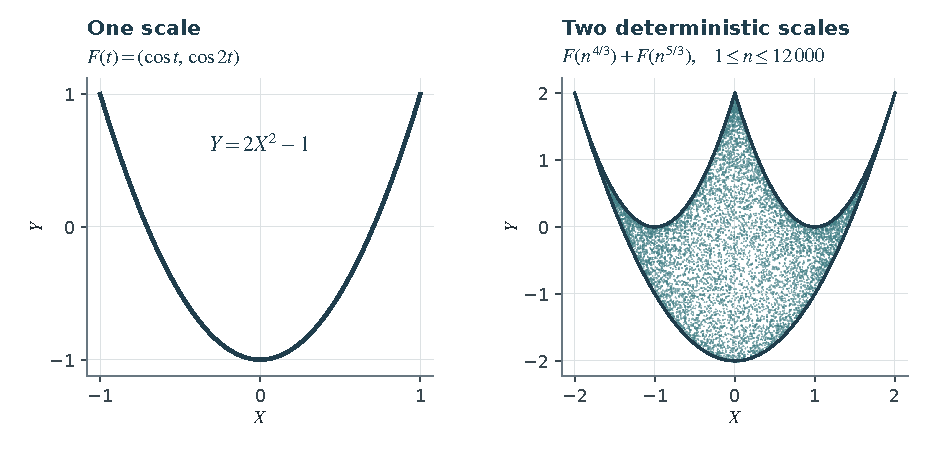
\includegraphics[width=.94\linewidth]{resonant-model.pdf}
\caption{A fully resonant model in two dimensions. One observation lies on \(y=2x^2-1\). The right panel uses \(12{,}000\) deterministic sums at exponents \(4/3\) and \(5/3\). Writing \(x=u+v,\ y=2(u^2+v^2)-2\) with \(u,v\in[-1,1]\) gives the two exact support boundaries shown. The plotted points illustrate the general sharpness example.}\label{fig:model}
\end{figure}

\begin{corollary}[Orderings in pooled centered races]\label{cor:order}
Let \(M=\int x\dd\mu_X(x)\). For each \(m\), choose \(\alpha_j=1+j/(m+1)\). The limiting frequency as \(n\to\infty\) of each strict coordinate ordering of \(S_n-mM\) exists. As \(m\to\infty\), it tends to the probability of the same ordering for a centered Gaussian with covariance \(\operatorname{Cov}(\mu_X)\). In particular every ordering occurs with positive limiting frequency for all sufficiently large fixed \(m\).
\end{corollary}
\begin{proof}
The boundary of an ordering cone is contained in a finite union of tie hyperplanes. Each has zero mass under any convolution by Theorem~\ref{th:local}. That theorem also gives strictly positive variance in every nonzero direction. Apply the multivariate central limit theorem to independent vectors with law \(\mu_X\); the convolution identity transfers the result to \eqref{eq:Sn}. A nondegenerate Gaussian assigns positive probability to each strict ordering and zero probability to its boundary. There are only finitely many orderings for fixed \(q\).
\end{proof}

\section{An explicit exponent for broad Gaussian windows}
\label{sec:broad}
Write the centered Gaussian-smoothed limiting vector in the form
\[
   Y_h(z)=2\operatorname{Re}\sum_{\gamma>0}
                   e^{-h\gamma^2} b_\gamma z_\gamma ,
       \qquad h>0,
\]
where $z$ is Haar distributed on the closure of the orbit
$(e^{i\gamma t})_{\gamma>0}$. The vectors $b_\gamma\in\mathbb C^d$
are the unsmoothed coefficients, with coincident ordinates grouped.
Thus $Y_h=F_z(0)-b_0$ in the notation of the prime-power formula.
A common time translation leaves the law unchanged. The sum of
$\|b_\gamma\|$ over $0<\gamma\le T$ is $O_q((1+T)\log(2+T))$ for
the vectors $b_\gamma(a)=-d^{-1}\sum_\chi
\overline{\chi(a)}m_\chi(\gamma)$.

In increasing order of $\gamma$, retain $\gamma$ if adjoining
$\operatorname{Re}b_\gamma$ and $\operatorname{Im}b_\gamma$ increases
the dimension of the real span. Write $\lambda_1<\cdots<\lambda_r$
for the retained ordinates. The zero-divisor independence lemma implies
that this span eventually equals $\mathbb R^d$, so $1\le r\le d$.
For any nonzero real vector $v$ put
\[
 A_h(v)=\max_{1\le j\le r}e^{-h\lambda_j^2}
                         |v\cdot b_{\lambda_j}|>0 .
\]
Here the dot product extends the real dot product complex-linearly in
the second argument.

\begin{theorem}\label{thm:broad}
There are $h_0$ and $C$, depending only on this spectrum, such that
for $h\ge h_0$, every nonzero $v$, and every Borel $E\subset\mathbb R$,
\[
  \Pr\{v\cdot Y_h\in E\}
    \le \min\left\{1,\;C\left(\frac{|E|}{A_h(v)}\right)^{1/(2r)}\right\}.
\]
The characteristic function in this direction satisfies
\[
 \left|\mathbb E\exp(iu\,v\cdot Y_h)\right|
       \le C(1+|u|A_h(v))^{-1/(2r)} .
\]
In particular $1/(2d)$ is always an admissible exponent.
\end{theorem}

The directional normalization is necessary for a bound uniform in $h$,
since every centered projection tends to zero as $h\to\infty$.

\begin{proof}
Along any orbit translate, divide the scalar projection by $A_h(v)$.
Its retained part is a trigonometric polynomial at the fixed $2r$
frequencies $\nu\in\{\pm\lambda_1,\ldots,\pm\lambda_r\}$.
At least one of its complex coefficients has modulus one and all
have modulus at most one. At every time, the vector of its derivatives
of orders $1,\ldots,2r$ is the matrix $((i\nu)^k)_{k,\nu}$ times
the vector of its phased coefficients. Factoring $i\nu$ from each column leaves an invertible Vandermonde matrix.
The maximum of these derivative moduli is therefore bounded below
by a positive constant depending only on the retained ordinates.

For an omitted $\gamma$, the two real vectors
$\operatorname{Re}b_\gamma$ and $\operatorname{Im}b_\gamma$ belong
to the span at the preceding retained stage. Choose once and for
all a basis from the retained vectors at each of the finitely many
stages. Boundedness of each coordinate map gives
\[
 \frac{e^{-h\gamma^2}|v\cdot b_\gamma|}{A_h(v)}
 \le C_q\|b_\gamma\|\!
        \sum_{j:\lambda_j<\gamma}
                    e^{-h(\gamma^2-\lambda_j^2)} .
\]
For $h\ge1$, the right side times $(1+\gamma)^{2r+1}$ has a summable
majorant. Every term tends to zero, so the omitted part tends uniformly
to zero with all derivatives through order $2r+1$, uniformly in
$v$ and in the phases. For $h$ sufficiently large the normalized
function thus has some derivative of order $1,\ldots,2r$ bounded
away from zero at every point, and all derivatives through order
$2r+1$ are bounded above uniformly. The one-dimensional finite-type
estimates, applied on unit orbit segments and averaged over Haar
measure, give the asserted bounds.
\end{proof}

For each fixed $h\ge h_0$, the late unit-interval estimates for the
arithmetic signal have the same exponent after division by $A_h(v)$.
To see this, normalize $\|v\|=1$. The map $v\mapsto A_h(v)$ is continuous
and positive on the unit sphere, so its minimum is positive for this
fixed $h$. The differentiated explicit-formula remainder through order
$2r+1$ is consequently $o(1)$ even after division by $A_h(v)$, uniformly
over such $v$ as the left endpoint $T$ tends to infinity. The threshold
on $T$ in this assertion may depend on $h$.

\begin{corollary}[One projected oscillation at broad bandwidth]
For fixed $v\ne0$, let $\gamma_* >0$ be the first frequency such that
$v\cdot b_{\gamma_*}\ne0$. Then
\[
 \frac{v\cdot Y_h}{2e^{-h\gamma_*^2}|v\cdot b_{\gamma_*}|}
       \ \xrightarrow[h\to\infty]{\mathrm{law}}\ \cos\Theta,\qquad
       \Theta\ \text{uniform on }[0,2\pi].
\]
\end{corollary}

\begin{proof}
The projection of the phase group on this frequency is the
whole circle and the normalized tail converges uniformly to zero.
If $\gamma'>\gamma_*$ is the next contributing frequency, this coupling
has error $O_{q,v}(e^{-h((\gamma')^2-\gamma_*^2)})$ for $h\ge1$.
The limiting density $1/(\pi\sqrt{1-y^2})$ on $(-1,1)$ assigns mass
of order $\sqrt\varepsilon$ to $[1-\varepsilon,1]$. In the scalar
case the exponent $1/2$ is consequently sharp for bounds uniform
as $h\to\infty$.
\end{proof}

\begin{corollary}[Counting crossings of a smoothed prime statistic]
\label{cor:crossings}
Fix a nonzero real $v$. For all sufficiently large fixed $h$, the
number of crossings of its own limiting mean by either scalar arithmetic
statistic $v\cdot \mathcal P(t)$ or $v\cdot \mathcal Q(t)$ in the
log-time interval $[0,T]$ equals
\[
                    \frac{\gamma_*}{\pi}T+O_{q,v,h}(1).
\]
Every sufficiently late crossing is simple. If
$\phi=\arg(v\cdot b_{\gamma_*})$, there is exactly one crossing near
each sufficiently late point $(\pi/2+k\pi-\phi)/\gamma_*$.
\end{corollary}

\begin{proof}
Set $\theta=\gamma_*t+\phi$, subtract the limiting mean of the
chosen scalar statistic, and divide by
$2e^{-h\gamma_*^2}|v\cdot b_{\gamma_*}|$.
In this coordinate the first oscillation is $\cos\theta$. The sum of
all higher oscillations and its first derivative tend uniformly to
zero with $h$, by the preceding tail estimate with an extra weight
$1+\gamma/\gamma_*$. For fixed sufficiently large $h$, the additional
arithmetic remainder and its derivative tend to zero with $t$. The two
errors together can therefore be bounded in modulus, separately for
derivative and value, by $1/4$ for all sufficiently late times.
Outside the intervals $|\theta-(\pi/2+k\pi)|<\pi/6$ we have
$|\cos\theta|\ge1/2$. Inside each interval, $|\sin\theta|\ge\sqrt3/2$;
the perturbed cosine is strictly monotone there and has opposite signs
at the endpoints. Each such interval contributes exactly one simple
crossing. The arithmetic statistic is real analytic and nonconstant,
so a bounded initial interval contributes finitely many crossings.
\end{proof}


\section{Further research questions}
\begin{enumerate}[leftmargin=*]
\item At \(h=h_*\), does the actual modulo-four race ever return below zero at arbitrarily large times? This asks how rapidly phases return to a minimizer relative to the prime-square error.
\item Is the Gaussian transition exactly the solution of \(2\sum_{\gamma>0}m_\gamma \e^{-h\gamma^2}=1/2\)? It suffices that the all-minus phase lies in the beta-zero orbit closure. The certificate uses one near-minimizing time.
\item What is the true asymptotic of the losing density as \(h\uparrow h_*\)? Estimate \eqref{eq:rate} uses only local curvature in one time direction. Several effective independent phase directions could give a faster rate.
\item For each \(q\), what is the smallest number of scales in \eqref{eq:Sn} that yields a full-dimensional density for primes? Our upper bound is \(d=\varphi(q)\). Improving this bound requires more information about the zero ordinates.
\end{enumerate}

\begin{thebibliography}{99}\small\setlength{\itemsep}{0.5pt}\setlength{\parsep}{0pt}\setlength{\parskip}{0pt}
\bibitem{sernau} L. Sernau and collaborators, \emph{GRH for Dirichlet L-functions, in Lean 4}, commit \texttt{72fead102f66}. \href{https://github.com/lsernau/grh-lean/tree/72fead102f663d5c7a407964a13dc0cf9d977207}{Repository}; \href{https://github.com/lsernau/grh-lean/blob/72fead102f663d5c7a407964a13dc0cf9d977207/grh/src/Statements.lean}{statements}; \href{https://github.com/lsernau/grh-lean/blob/72fead102f663d5c7a407964a13dc0cf9d977207/grh/GUIDE.md}{proof guide}. A. V. Sutherland, \href{https://math.mit.edu/~drew/shortgrh/}{verification records for the shorter editions}.
\bibitem{lean} Lean FRO and Mathlib Initiative, \href{https://leanprover-community.github.io/blog/posts/riemann-hypothesis/}{\emph{Lean verification of the Riemann Hypothesis}}, 21 November 2026.
\bibitem{wiki} Wikipedia contributors, \href{https://en.wikipedia.org/wiki/Riemann_hypothesis}{\emph{Riemann hypothesis}}, consulted 26 November 2026.
\bibitem{proveit} V. Reshetnikov, \emph{ProveIt}, commit \texttt{041d80325417}. \href{https://github.com/VladimirReshetnikov/ProveIt/tree/041d8032541746f2ac2e686fbe437f8092771670/Analysis/GeneralizedRiemannHypothesis}{GRH collection}; \href{https://github.com/VladimirReshetnikov/ProveIt/blob/041d8032541746f2ac2e686fbe437f8092771670/Analysis/GeneralizedRiemannHypothesis/Article/sections/zer.tex}{section on zeros, multiplicity rank and prime races}.
\bibitem{banks} W. D. Banks, \href{https://arxiv.org/abs/2302.07073}{\emph{Comparing zeros of distinct Dirichlet \(L\)-functions}}, arXiv:2302.07073.
\bibitem{rs} M. Rubinstein and P. Sarnak, \href{https://doi.org/10.1080/10586458.1994.10504289}{\emph{Chebyshev's bias}}, Experimental Mathematics 3 (1994), 173--197.
\bibitem{ans} A. Akbary, N. Ng and M. Shahabi, \href{https://arxiv.org/abs/1306.1657}{\emph{Limiting distributions of the classical error terms of prime number theory}}, Quarterly Journal of Mathematics 65 (2014), 743--780.
\bibitem{devin} L. Devin, \href{https://doi.org/10.4153/S0008439520000089}{\emph{Limiting properties of the distribution of primes in an arbitrarily large number of residue classes}}, Canadian Mathematical Bulletin 63 (2020), 837--849.
\bibitem{mn} G. Martin and N. Ng, \href{https://arxiv.org/abs/1710.00088}{\emph{Inclusive prime number races}}, Transactions of the American Mathematical Society (2020), DOI 10.1090/tran/7996.
\bibitem{lawton} W. Lawton, \href{https://arxiv.org/abs/1904.09373}{\emph{Distribution of small values of Bohr almost periodic functions with bounded spectrum}}, J. Siberian Federal University, Math.\ Phys.\ 12 (2019), 571--578.
\bibitem{ghs} I. Glazer, Y. I. Hendel and S. Sodin, \href{https://arxiv.org/abs/2202.12446}{\emph{Integrability of pushforward measures by analytic maps}}, arXiv:2202.12446.
\bibitem{kouk} D. Koukoulopoulos, \href{https://dms.umontreal.ca/~koukoulo/documents/publications/primes.pdf}{\emph{The Distribution of Prime Numbers}}, AMS, Chapters 11--12; and H. Davenport, \emph{Multiplicative Number Theory}, 3rd ed., Springer, Chapters 12--16.
\bibitem{gk} S. W. Graham and G. Kolesnik, \emph{Van der Corput's Method of Exponential Sums}, Cambridge University Press, 1991, Chapter 2.
\bibitem{kt} S. Knapowski and P. Tur\'an, \emph{\"Uber einige Fragen der vergleichenden Primzahltheorie}, in \emph{Number Theory and Analysis}, Plenum, 1969, 157--171. The moving Gaussian result is also stated in \cite[eq.~(5)]{bp} and \cite[after eq.~(17)]{suzuki}.
\bibitem{bp} H.-J. Bentz and J. Pintz, \href{https://personal.math.ubc.ca/~gerg/teaching/592-Fall2018/papers/1980.Bentz.pdf}{\emph{Quadratic residues and the distribution of prime numbers}}, Monatshefte f\"ur Mathematik 90 (1980), 91--100.
\bibitem{suzuki} M. Suzuki, \href{https://doi.org/10.1007/s11139-025-01238-9}{\emph{On variants of Chebyshev's conjecture}}, Ramanujan Journal (2025).
\bibitem{neroli} Z. Neroli, \href{https://arxiv.org/abs/2611.32862}{\emph{On the Fujii conjectures}}, arXiv:2611.32862, 24 November 2026, Thms. 2.2 and 3.3.
\end{thebibliography}

\end{document}
